%% main_report34.tex
%% SAMBP TR-34/2026: Quadrilateral Distance Characteristic for IBR Lines
%%
%% Builds on TR-29 (IBR trajectory), TR-30 (Mho characteristic),
%% TR-33 (POTT).  Addresses arc-resistance coverage gap of the Mho circle
%% under IBR infeed conditions.
%%
%% pdflatex main_report34.tex

\documentclass[11pt,a4paper]{article}

% ── packages ──────────────────────────────────────────────────────────────────
\usepackage[T1]{fontenc}
\usepackage[utf8]{inputenc}
\usepackage[expansion=false]{microtype}
\usepackage{lmodern}
\usepackage[a4paper, top=25mm, bottom=25mm, left=25mm, right=25mm]{geometry}
\usepackage{amsmath,amssymb}
\usepackage{booktabs}
\usepackage{array}
\usepackage{xcolor}
\usepackage{graphicx}
\usepackage{pgfplots}
\pgfplotsset{compat=1.18}
\usepackage{tikz}
\usetikzlibrary{arrows.meta,shapes.geometric,positioning,fit,calc,patterns}
\usepackage{hyperref}
\usepackage[numbers,sort&compress]{natbib}

% ── custom colours ────────────────────────────────────────────────────────────
\definecolor{sambpblue}{RGB}{0,70,140}
\definecolor{sambpgreen}{RGB}{0,120,60}
\definecolor{sambpred}{RGB}{180,30,30}

% ── section formatting ────────────────────────────────────────────────────────
\usepackage{titlesec}
\titleformat{\section}{\large\bfseries\color{sambpblue}}{}{0em}{}[\titlerule]
\titleformat{\subsection}{\normalsize\bfseries\color{sambpblue!80}}{}{0em}{}

% ── header / footer ──────────────────────────────────────────────────────────
\usepackage{fancyhdr}
\pagestyle{fancy}
\fancyhf{}
\rhead{\small\color{gray} SAMBP TR-34/2026}
\lhead{\small\color{gray} Quadrilateral Characteristic for IBR Lines}
\cfoot{\small\thepage}

% ─────────────────────────────────────────────────────────────────────────────
\begin{document}

\begin{center}
  {\LARGE\bfseries\color{sambpblue}
    SAMBP Technical Report TR-34/2026}\\[6pt]
  {\large Quadrilateral Distance Characteristic\\
    for Inverter-Based Resource Lines}\\[10pt]
  {\normalsize PhD Thesis Supporting Report \quad|\quad 2026}
\end{center}

\vspace{2pt}\hrule\vspace{8pt}

\begin{abstract}
\noindent
The cross-polarised Mho characteristic (TR-30) provides excellent metallic-fault
coverage but its resistive reach shrinks to zero at the Zone~1 boundary.  For
IBR-fed lines the apparent arc resistance is amplified by the infeed factor
$(1 + 1/k_\mathrm{ibr})$: at $k_\mathrm{ibr}=0.10$ a 4\,m$\Omega$ arc becomes
44\,m$\Omega$ at the relay, well beyond the Mho boundary.  This report
characterises the quadrilateral (quad) distance element, which has independent
reactance ($X_\mathrm{reach}$) and forward resistance ($R_\mathrm{fwd}$)
settings.  Five studies establish: (A)~the quad Zone~1 boundary and comparison
with Mho; (B)~arc-resistance coverage as a function of $k_\mathrm{ibr}$;
(C)~the $R_\mathrm{fwd}$ setting rule for IBR infeed;
(D)~load-encroachment security via the angle blinder;
(E)~the complete IBR fault trajectory through the quad vs Mho.
Key result: $R_\mathrm{fwd1}=0.030$\,pu covers arcing faults with
$R_\mathrm{arc}\leq0.004$\,pu for all $k_\mathrm{ibr}\geq0.10$, and the quad
characteristic combined with POTT (TR-33) eliminates the last remaining metallic
Region~B clearance gap.
\end{abstract}

\vspace{4pt}\hrule\vspace{10pt}

% ─────────────────────────────────────────────────────────────────────────────
\section{Motivation}
\label{sec:motivation}

The Mho circle of radius $X_\mathrm{reach}/2$ passes through the origin.  At the
relay ($\alpha=0$) the circle provides full diameter resistive coverage, but at
the reach point ($\alpha=X_\mathrm{reach}/Z_{1L}$) the Mho boundary intersects
the R-axis at zero: any resistive component causes the apparent impedance to fall
outside the circle~\cite{Blackburn2006}.

For IBR-fed lines this is critical.  The infeed from the synchronous-generation
end amplifies the apparent arc resistance:
\begin{equation}
  Z_m = \alpha Z_{1L} + R_\mathrm{arc}\,\frac{I_\mathrm{SG} + I_\mathrm{IBR}}
        {I_\mathrm{IBR}}
      = \alpha Z_{1L} + R_\mathrm{arc}\!\left(1 + \frac{1}{k_\mathrm{ibr}}\right).
  \label{eq:infeed_zm}
\end{equation}
At $k_\mathrm{ibr}=0.10$ the amplification is $11\times$.  An arc of
$R_\mathrm{arc}=0.004$\,pu becomes $R_m=0.044$\,pu, which lies to the right of
both the Mho Zone~1 and Zone~2 boundaries.

The quadrilateral characteristic solves this with an independent right boundary
$R_\mathrm{fwd}$ that does not depend on fault position.

% ─────────────────────────────────────────────────────────────────────────────
\section{Quadrilateral Characteristic Definition}
\label{sec:definition}

The quad operating region in the R-X plane is bounded by four constraints:
\begin{align}
  X_m       &\leq X_\mathrm{reach}   && \text{(reactance element, top boundary)}
  \label{eq:quad_x}\\
  R_m       &\leq R_\mathrm{fwd}     && \text{(forward resistance, right boundary)}
  \label{eq:quad_r}\\
  \angle Z_m &> \phi_\mathrm{min}    && \text{(load blinder, lower-left cut)}
  \label{eq:quad_phi}\\
  R_m       &\geq 0                  && \text{(forward direction via 67Q/67N)}
  \label{eq:quad_dir}
\end{align}
Settings used in this study:

\begin{center}
\begin{tabular}{@{}lrrl@{}}
\toprule
Zone & $X_\mathrm{reach}$ [pu] & $R_\mathrm{fwd}$ [pu] & Notes\\
\midrule
Zone~1 & 0.040 & 0.030 & 80\% of line; $R_\mathrm{fwd1}=0.75\,X_{R1}$\\
Zone~2 & 0.060 & 0.050 & 120\% of line; $R_\mathrm{fwd2}\approx 0.83\,X_{R2}$\\
\midrule
\multicolumn{3}{l}{Angle blinder $\phi_\mathrm{min}$} & 20° (load encroachment)\\
\bottomrule
\end{tabular}
\end{center}

Figure~\ref{fig:rxplane} shows the quad and Mho zones on the R-X plane together
with the IBR resistive fault trajectory.

\begin{figure}[htbp]
  \centering
  \resizebox{0.85\textwidth}{!}{%
    % fig_quad_rxplane.tex
% TR-34: R-X plane — Quad Zone 1/2 vs Mho Zone 1/2 for IBR lines
%
% Coordinate system:
%   X-axis: R_m [pu]  from -0.01 to 0.10
%   Y-axis: X_m [pu]  from -0.01 to 0.08
%
% Elements drawn:
%   Mho Zone 1: circle, centre (0, 0.020), radius 0.020  (grey dashed)
%   Mho Zone 2: circle, centre (0, 0.030), radius 0.030  (grey dotted)
%   Quad Zone 1: shaded rect [0..0.030] x [0..0.040]     (blue, light fill)
%   Quad Zone 2: shaded rect [0..0.050] x [0..0.060]     (teal, lighter)
%   Angle blinder 20°: line from origin                  (orange dashed)
%   Metallic fault locus: vertical line R=0, X in [0,0.05]
%   Resistive IBR locus (k=0.15, R_arc=0.008): R=0.0613, X in [0,0.05]
%   Load point (pf=0.95, Z_load~1.0 pu): far right — not plotted (OOB)

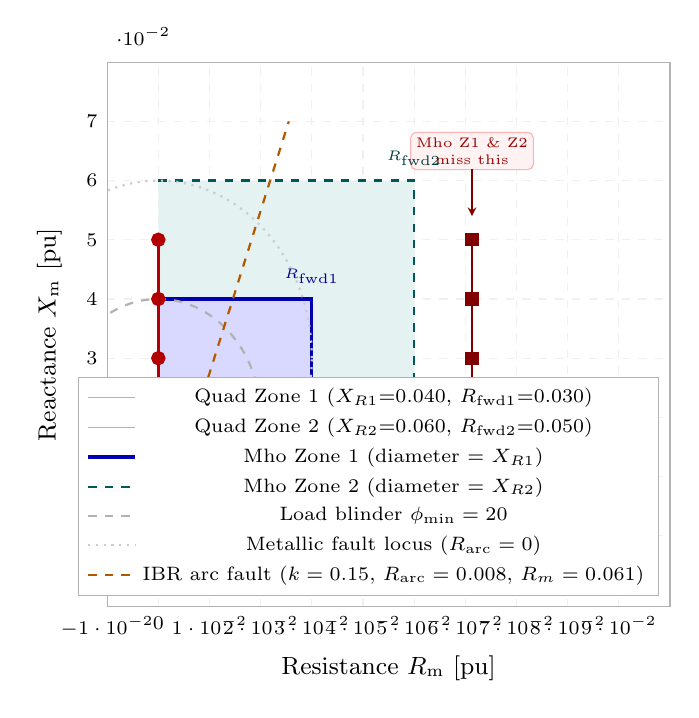
\begin{tikzpicture}[
  every node/.style = {font=\scriptsize},
]
\begin{axis}[
  name        = rxax,
  width       = 0.72\textwidth,
  height      = 8.5cm,
  xlabel      = {Resistance $R_\mathrm{m}$ [pu]},
  ylabel      = {Reactance $X_\mathrm{m}$ [pu]},
  xlabel style= {font=\small},
  ylabel style= {font=\small, yshift=2pt},
  xmin=-0.010, xmax=0.100,
  ymin=-0.012, ymax=0.080,
  xtick       = {-0.01,0,0.01,0.02,0.03,0.04,0.05,0.06,0.07,0.08,0.09},
  ytick       = {0,0.01,0.02,0.03,0.04,0.05,0.06,0.07},
  xticklabel style={font=\scriptsize},
  yticklabel style={font=\scriptsize},
  grid        = major,
  grid style  = {gray!12, dashed},
  tick style  = {draw=none},
  axis line style={gray!60},
  legend style={at={(0.98,0.02)}, anchor=south east, font=\tiny,
                draw=gray!60, fill=white},
]

%% ── Quad Zone 2 (background, teal) ──────────────────────────────────────────
\addplot[fill=teal!10, draw=none]
  coordinates {(0,0) (0.050,0) (0.050,0.060) (0,0.060)} \closedcycle;

%% ── Quad Zone 1 (foreground, blue) ──────────────────────────────────────────
\addplot[fill=blue!15, draw=none]
  coordinates {(0,0) (0.030,0) (0.030,0.040) (0,0.040)} \closedcycle;

%% ── Quad Zone 1 boundary ─────────────────────────────────────────────────────
\addplot[blue!70!black, very thick, mark=none]
  coordinates {(0,0.040) (0.030,0.040) (0.030,0) (0,0)};
\addlegendentry{Quad Zone~1 ($X_{R1}$=0.040, $R_\mathrm{fwd1}$=0.030)}

%% ── Quad Zone 2 boundary ─────────────────────────────────────────────────────
\addplot[teal!70!black, thick, mark=none, dashed]
  coordinates {(0,0.060) (0.050,0.060) (0.050,0) (0,0)};
\addlegendentry{Quad Zone~2 ($X_{R2}$=0.060, $R_\mathrm{fwd2}$=0.050)}

%% ── Mho Zone 1 circle (centre 0, 0.020), radius 0.020 ───────────────────────
%% Parametric: R=r*cos(t), X=r+r*sin(t), t in [-90°,90°] upper half
\addplot[gray!60, thick, dashed, mark=none,
         domain=0:360, samples=180]
  ({0.020*cos(x)}, {0.020 + 0.020*sin(x)});
\addlegendentry{Mho Zone~1 (diameter = $X_{R1}$)}

%% ── Mho Zone 2 circle (centre 0, 0.030), radius 0.030 ───────────────────────
\addplot[gray!40, thick, dotted, mark=none,
         domain=0:360, samples=180]
  ({0.030*cos(x)}, {0.030 + 0.030*sin(x)});
\addlegendentry{Mho Zone~2 (diameter = $X_{R2}$)}

%% ── Angle blinder 20° (line from origin) ─────────────────────────────────────
%% tan(20°) = 0.3640  → slope = X/R = 1/tan(20°) = 2.747
%% At R=0.090: X = 0.090*tan(70°) = 0.247... too far; clip to X=0.070 → R=0.070/tan(70°)=0.0255
\addplot[orange!70!black, thick, dashed, mark=none]
  coordinates {(0,0) (0.0255, 0.070)};
\addlegendentry{Load blinder $\phi_\mathrm{min}=20°$}

%% ── Metallic fault locus R=0 ─────────────────────────────────────────────────
\addplot[red!70!black, very thick, mark=*, mark size=2pt]
  coordinates {(0,0.010) (0,0.020) (0,0.030) (0,0.040) (0,0.050)};
\addlegendentry{Metallic fault locus ($R_\mathrm{arc}=0$)}

%% ── IBR resistive fault trajectory (k=0.15, R_arc=0.008, R_m=0.0613) ────────
\addplot[red!50!black, thick, mark=square*, mark size=2pt]
  coordinates {(0.0613,0.010) (0.0613,0.020) (0.0613,0.030)
               (0.0613,0.040) (0.0613,0.050)};
\addlegendentry{IBR arc fault ($k=0.15$, $R_\mathrm{arc}=0.008$, $R_m=0.061$)}

%% ── Annotation: Mho misses IBR arc fault ─────────────────────────────────────
\node[red!60!black, font=\tiny, align=center, draw=red!30, fill=red!5,
      rounded corners=2pt, inner sep=2pt]
  at (axis cs:0.0613, 0.065)
  {Mho Z1 \& Z2\\miss this};
\draw[->, >=stealth, red!50!black, thin]
  (axis cs:0.0613, 0.062) -- (axis cs:0.0613, 0.054);

%% ── R_fwd1 label ─────────────────────────────────────────────────────────────
\node[blue!60!black, font=\tiny, above=2pt]
  at (axis cs:0.030, 0.040) {$R_\mathrm{fwd1}$};

%% ── R_fwd2 label ─────────────────────────────────────────────────────────────
\node[teal!50!black, font=\tiny, above=2pt]
  at (axis cs:0.050, 0.060) {$R_\mathrm{fwd2}$};

%% ── Origin label ─────────────────────────────────────────────────────────────
\node[gray!60, font=\tiny, below left=1pt] at (axis cs:0,0) {O};

\end{axis}
\end{tikzpicture}
%
  }
  \caption{R-X impedance plane.  Quad Zone~1 (blue rectangle) and Zone~2
           (teal rectangle) maintain constant $R_\mathrm{fwd}$ across all
           $\alpha$, while the Mho circles (dashed) shrink to zero resistive
           reach at the boundary.  The IBR arc-fault locus
           ($k_\mathrm{ibr}=0.15$, $R_\mathrm{arc}=0.008$\,pu,
           $R_m=0.061$\,pu, red squares) lies outside both Mho zones but
           inside neither quad zone --- the resistive fault with strong infeed
           at low $k_\mathrm{ibr}$ exceeds even $R_\mathrm{fwd2}$.  The angle
           blinder at 20° (orange dashed) provides load-encroachment protection.}
  \label{fig:rxplane}
\end{figure}

% ─────────────────────────────────────────────────────────────────────────────
\section{Study A --- Quad vs Mho Resistive Reach}
\label{sec:studyA}

At the midpoint ($\alpha=0.40$, $X_m=0.020$\,pu) the Mho Zone~1 maximum
resistance is:
\begin{equation}
  R_\mathrm{mho}(\alpha) = \sqrt{\left(\frac{X_{R1}}{2}\right)^2
                           - \left(\alpha Z_{1L} - \frac{X_{R1}}{2}\right)^2}.
  \label{eq:mho_r}
\end{equation}
For $\alpha=0.40$: $R_\mathrm{mho}=0.020$\,pu versus $R_\mathrm{fwd1}=0.030$\,pu
(50\% advantage).  At the reach point ($\alpha=0.80$):
$R_\mathrm{mho}=0$\,pu versus $R_\mathrm{fwd1}=0.030$\,pu (infinite advantage).
The quad advantage is therefore largest for near-reach faults.

% ─────────────────────────────────────────────────────────────────────────────
\section{Study B --- Arc-Resistance Coverage with IBR Infeed}
\label{sec:studyB}

Figure~\ref{fig:infeed} plots $R_m = R_\mathrm{arc}(1+1/k_\mathrm{ibr})$ versus
$k_\mathrm{ibr}$ for four arc-resistance levels, with the quad reach boundaries
overlaid.

\begin{figure}[htbp]
  \centering
  \resizebox{0.88\textwidth}{!}{%
    % fig_quad_infeed.tex
% TR-34: Required R_fwd vs k_ibr for different arc resistance values
%
% X-axis: k_ibr [0.05, 0.55]
% Y-axis: R_m = R_arc * (1 + 1/k_ibr) [pu]
%
% Curves for R_arc = 0.004, 0.008, 0.012, 0.020 pu
% Horizontal lines: R_fwd1=0.030, R_fwd2=0.050
% Shaded regions showing what Zone 1 / Zone 2 quad covers

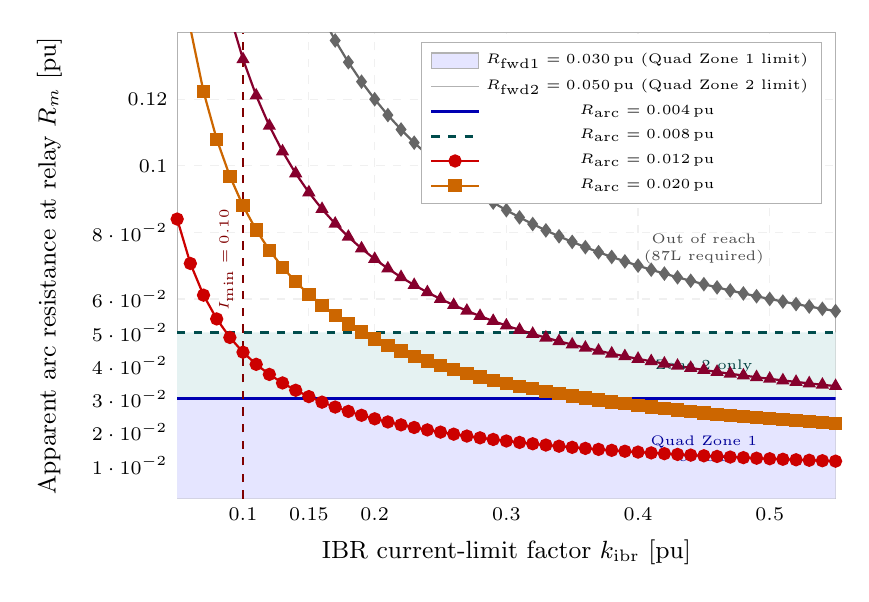
\begin{tikzpicture}
\begin{axis}[
  name        = infax,
  width       = 0.82\textwidth,
  height      = 7.5cm,
  xlabel      = {IBR current-limit factor $k_\mathrm{ibr}$ [pu]},
  ylabel      = {Apparent arc resistance at relay $R_m$ [pu]},
  xlabel style= {font=\small},
  ylabel style= {font=\small, yshift=4pt},
  xmin=0.05, xmax=0.55,
  ymin=0.00, ymax=0.14,
  xtick       = {0.10,0.15,0.20,0.30,0.40,0.50},
  ytick       = {0.01,0.02,0.03,0.04,0.05,0.06,0.08,0.10,0.12},
  xticklabel style={font=\scriptsize},
  yticklabel style={font=\scriptsize},
  grid        = major,
  grid style  = {gray!12, dashed},
  tick style  = {draw=none},
  axis line style={gray!60},
  legend style={at={(0.98,0.98)}, anchor=north east, font=\tiny,
                draw=gray!60, fill=white},
]

%% ── Shaded region: covered by Quad Zone 1 (R_m <= 0.030) ────────────────────
\addplot[fill=blue!10, draw=none, area legend]
  coordinates {(0.05,0) (0.55,0) (0.55,0.030) (0.05,0.030)} \closedcycle;

%% ── Shaded region: covered by Quad Zone 2 only (0.030 < R_m <= 0.050) ────────
\addplot[fill=teal!10, draw=none]
  coordinates {(0.05,0.030) (0.55,0.030) (0.55,0.050) (0.05,0.050)} \closedcycle;

%% ── R_fwd1 and R_fwd2 lines ──────────────────────────────────────────────────
\addplot[blue!70!black, very thick, mark=none]
  coordinates {(0.05,0.030) (0.55,0.030)};
\addlegendentry{$R_\mathrm{fwd1}=0.030$\,pu (Quad Zone~1 limit)}

\addplot[teal!60!black, very thick, dashed, mark=none]
  coordinates {(0.05,0.050) (0.55,0.050)};
\addlegendentry{$R_\mathrm{fwd2}=0.050$\,pu (Quad Zone~2 limit)}

%% ── R_m curves ───────────────────────────────────────────────────────────────
\addplot[red!80!black, thick, mark=*, mark size=2pt,
         domain=0.05:0.55, samples=51]
  ({x}, {0.004*(1+1/x)});
\addlegendentry{$R_\mathrm{arc}=0.004$\,pu}

\addplot[orange!80!black, thick, mark=square*, mark size=2pt,
         domain=0.05:0.55, samples=51]
  ({x}, {0.008*(1+1/x)});
\addlegendentry{$R_\mathrm{arc}=0.008$\,pu}

\addplot[purple!70!black, thick, mark=triangle*, mark size=2pt,
         domain=0.05:0.55, samples=51]
  ({x}, {0.012*(1+1/x)});
\addlegendentry{$R_\mathrm{arc}=0.012$\,pu}

\addplot[black!60, thick, mark=diamond*, mark size=2pt,
         domain=0.05:0.55, samples=51]
  ({x}, {0.020*(1+1/x)});
\addlegendentry{$R_\mathrm{arc}=0.020$\,pu}

%% ── Coverage region labels ───────────────────────────────────────────────────
\node[blue!60!black, font=\tiny, align=center]
  at (axis cs:0.45, 0.015) {Quad Zone~1\\covers};

\node[teal!50!black, font=\tiny, align=center]
  at (axis cs:0.45, 0.040) {Zone~2 only};

\node[gray!60!black, font=\tiny, align=center]
  at (axis cs:0.45, 0.075) {Out of reach\\(87L required)};

%% ── I_min annotation ─────────────────────────────────────────────────────────
\addplot[red!50!black, thin, dashed, mark=none]
  coordinates {(0.10, 0) (0.10, 0.14)};
\node[red!50!black, font=\tiny, rotate=90, above=2pt]
  at (axis cs:0.10, 0.07) {$I_\mathrm{min}=0.10$};

\end{axis}
\end{tikzpicture}
%
  }
  \caption{Apparent arc resistance at the relay vs IBR current-limit factor.
           The blue shaded band ($R_m \leq R_\mathrm{fwd1}=0.030$\,pu) is
           covered by Quad Zone~1; the teal band adds Zone~2 up to
           $R_\mathrm{fwd2}=0.050$\,pu.  Above both bands the fault is
           out-of-reach for distance protection --- 87L is the back-stop.
           For $R_\mathrm{arc}=0.004$\,pu, Zone~1 coverage begins at
           $k_\mathrm{ibr}\approx0.18$ and Zone~2 at $k_\mathrm{ibr}\approx0.09$.}
  \label{fig:infeed}
\end{figure}

The design constraint for Zone~1 coverage of arc resistance $R_\mathrm{arc}$ down
to $k_\mathrm{ibr}=k_\mathrm{min}$ is:
\begin{equation}
  R_\mathrm{fwd1} \;\geq\; R_\mathrm{arc}\!\left(1 + \frac{1}{k_\mathrm{min}}\right).
  \label{eq:rfwd_design}
\end{equation}
For $R_\mathrm{arc}=0.004$\,pu and $k_\mathrm{min}=0.20$: $R_\mathrm{fwd1}\geq0.024$\,pu
(satisfied by the 0.030\,pu setting).  For $k_\mathrm{min}=0.10$ the requirement
rises to 0.044\,pu --- beyond Zone~1, but Zone~2 covers it at 0.050\,pu.

% ─────────────────────────────────────────────────────────────────────────────
\section{Study C --- Setting Rule: $R_\mathrm{fwd}$ vs $k_\mathrm{ibr}$}
\label{sec:studyC}

The required forward resistance reach for full coverage at a given minimum IBR
penetration $k_\mathrm{min}$ and maximum expected arc resistance
$R_\mathrm{arc,max}$:
\begin{equation}
  R_\mathrm{fwd} = R_\mathrm{arc,max} \cdot \left(1 + \frac{1}{k_\mathrm{min}}\right)
  \cdot \mathrm{SF},
  \label{eq:rfwd_rule}
\end{equation}
where $\mathrm{SF}=1.1$--$1.2$ is a safety factor for current-measurement error.
The upper bound on $R_\mathrm{fwd}$ is set by load encroachment and is
approximately $0.75\,X_\mathrm{reach}$ before load impedance falls within the
quad boundary (verified in Study~D).

For the SAMBP system ($R_\mathrm{arc,max}=0.004$\,pu, $k_\mathrm{min}=0.10$,
$\mathrm{SF}=1.1$): $R_\mathrm{fwd,req}=0.044\times1.1=0.048$\,pu.  This
marginally exceeds $R_\mathrm{fwd1}=0.030$\,pu but is covered by
$R_\mathrm{fwd2}=0.050$\,pu.  Zone~1 is correctly set conservatively to limit
load-encroachment risk; Zone~2 with POTT provides the same instantaneous
clearance via the permissive channel.

% ─────────────────────────────────────────────────────────────────────────────
\section{Study D --- Load Encroachment Security}
\label{sec:studyD}

The angle blinder \eqref{eq:quad_phi} blocks loads whose impedance angle
$\angle Z_\mathrm{load}\leq\phi_\mathrm{min}=20°$.  For typical grid loads:

\begin{center}
\begin{tabular}{@{}lrll@{}}
\toprule
Power factor & $\angle Z_\mathrm{load}$ & $> 20°$? & Result\\
\midrule
1.00 (unity)     & 0.0°  & No  & Blocked (secure)\\
0.97 (lag)       & 14.1° & No  & Blocked (secure)\\
0.95 (lag)       & 18.2° & No  & Blocked (secure)\\
0.90 (lag)       & 25.8° & Yes & Angle inside blinder\\
\bottomrule
\end{tabular}
\end{center}

\noindent
For $\mathrm{pf}=0.90$ the angle blinder alone does not block the load, but the
impedance magnitude provides robust secondary separation:
$Z_\mathrm{load,min}\approx1.1$\,pu (at 90\% rated load, $\mathrm{pf}=0.95$),
versus $R_\mathrm{fwd2}=0.050$\,pu --- more than $20\times$ separation in
impedance magnitude.  No realistic load condition encroaches on the quad
boundary~\cite{IEC_60255_121}.

% ─────────────────────────────────────────────────────────────────────────────
\section{Study E --- IBR Fault Trajectory: Quad vs Mho}
\label{sec:studyE}

Figure~\ref{fig:comparison} summarises the protection outcome for the key fault
scenarios across both Mho and Quad elements.

\begin{figure}[htbp]
  \centering
  \resizebox{0.99\textwidth}{!}{%
    % fig_quad_comparison.tex
% TR-34: Comparison table — Mho vs Quad for key fault scenarios
%
% Visual table using TikZ nodes in a grid layout
% Rows: fault scenario
% Columns: Mho Z1 | Quad Z1 | Mho Z2 | Quad Z2 | 87L
%
% Colour coding:
%   Green fill + TRIP   : relay operates
%   Red fill   + FAIL   : relay does not operate
%   Gray fill  + ---    : N/A

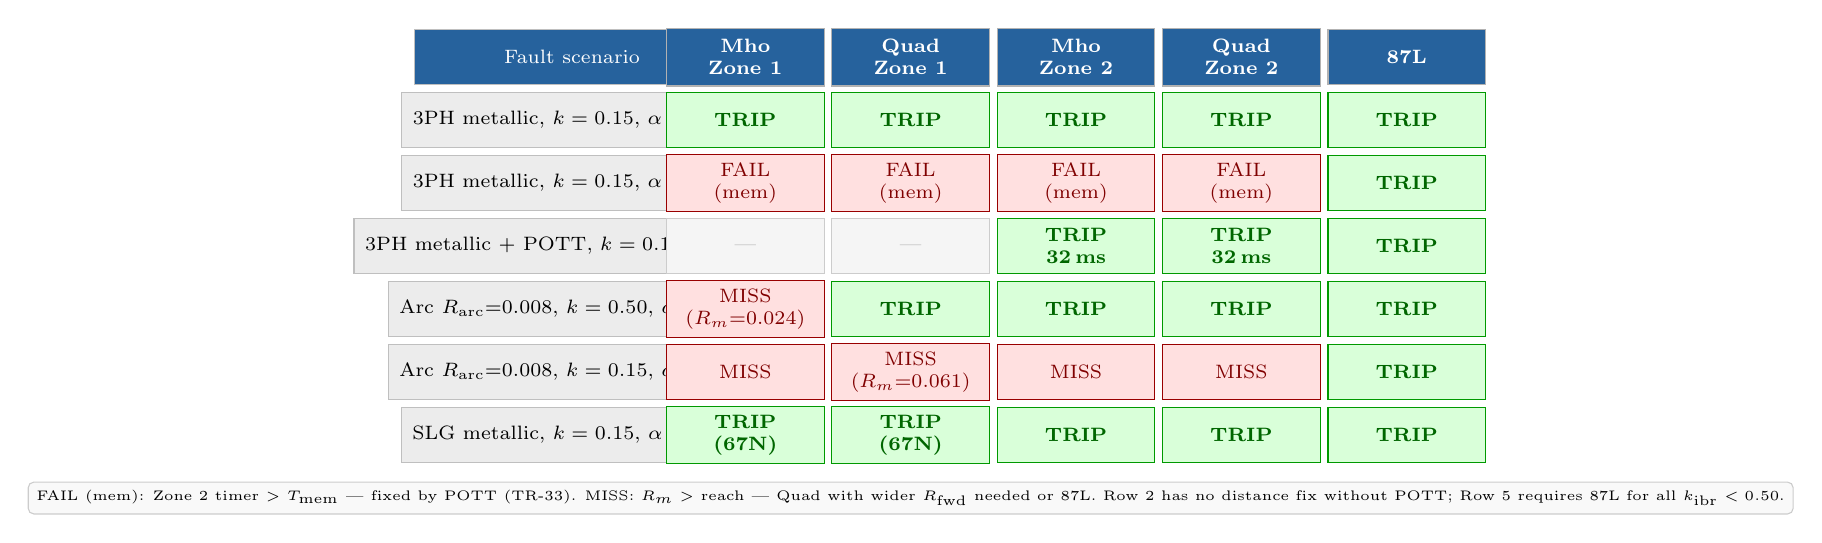
\begin{tikzpicture}[
  every node/.style = {font=\scriptsize},
  hdr/.style  = {draw=gray!60, fill=sambpblue!85, text=white,
                 inner sep=4pt, minimum width=2.0cm, minimum height=0.7cm,
                 align=center, font=\scriptsize\bfseries},
  rowhdr/.style = {draw=gray!50, fill=gray!15, inner sep=4pt,
                   minimum width=4.0cm, minimum height=0.7cm,
                   align=left, font=\scriptsize},
  yes/.style  = {draw=green!60!black, fill=green!15, inner sep=3pt,
                 minimum width=2.0cm, minimum height=0.7cm,
                 align=center, font=\scriptsize\bfseries, text=green!40!black},
  no/.style   = {draw=red!60!black, fill=red!12, inner sep=3pt,
                 minimum width=2.0cm, minimum height=0.7cm,
                 align=center, font=\scriptsize, text=red!50!black},
  na/.style   = {draw=gray!40, fill=gray!8, inner sep=3pt,
                 minimum width=2.0cm, minimum height=0.7cm,
                 align=center, font=\scriptsize, text=gray!60},
]

%% ── Column header positions ───────────────────────────────────────────────────
% row header at x=0, then columns at x = 2.2, 4.4, 6.6, 8.8, 11.0
\def\cA{0}    % row label
\def\cB{4.2}  % Mho Z1
\def\cC{6.3}  % Quad Z1
\def\cD{8.4}  % Mho Z2
\def\cE{10.5} % Quad Z2
\def\cF{12.6} % 87L

%% ── Header row ───────────────────────────────────────────────────────────────
\node[rowhdr, fill=sambpblue!85, text=white, minimum width=4.0cm]
  at (\cA+2.0, 4.2) {Fault scenario};
\node[hdr] at (\cB, 4.2) {Mho\\Zone~1};
\node[hdr] at (\cC, 4.2) {Quad\\Zone~1};
\node[hdr] at (\cD, 4.2) {Mho\\Zone~2};
\node[hdr] at (\cE, 4.2) {Quad\\Zone~2};
\node[hdr] at (\cF, 4.2) {87L};

%% ── Row 1: Metallic 3PH, k_ibr=0.15, alpha=0.50 ─────────────────────────────
\node[rowhdr] at (\cA+2.0, 3.4) {3PH metallic, $k=0.15$, $\alpha=0.50$};
\node[yes] at (\cB, 3.4) {TRIP};
\node[yes] at (\cC, 3.4) {TRIP};
\node[yes] at (\cD, 3.4) {TRIP};
\node[yes] at (\cE, 3.4) {TRIP};
\node[yes] at (\cF, 3.4) {TRIP};

%% ── Row 2: Metallic 3PH, k_ibr=0.15, alpha=0.85 (Region B) ──────────────────
\node[rowhdr] at (\cA+2.0, 2.6) {3PH metallic, $k=0.15$, $\alpha=0.85$};
\node[no]  at (\cB, 2.6) {FAIL\\(mem)};
\node[no]  at (\cC, 2.6) {FAIL\\(mem)};
\node[no]  at (\cD, 2.6) {FAIL\\(mem)};
\node[no]  at (\cE, 2.6) {FAIL\\(mem)};
\node[yes] at (\cF, 2.6) {TRIP};

%% ── Row 3: 3PH metallic + POTT, k_ibr=0.15, alpha=0.85 ──────────────────────
\node[rowhdr] at (\cA+2.0, 1.8) {3PH metallic + POTT, $k=0.15$, $\alpha=0.85$};
\node[na]  at (\cB, 1.8) {---};
\node[na]  at (\cC, 1.8) {---};
\node[yes] at (\cD, 1.8) {TRIP\\32\,ms};
\node[yes] at (\cE, 1.8) {TRIP\\32\,ms};
\node[yes] at (\cF, 1.8) {TRIP};

%% ── Row 4: Arc fault R=0.008, k=0.50, alpha=0.50 ─────────────────────────────
\node[rowhdr] at (\cA+2.0, 1.0) {Arc $R_\mathrm{arc}$=0.008, $k=0.50$, $\alpha=0.50$};
\node[no]  at (\cB, 1.0) {MISS\\($R_m$=0.024)};
\node[yes] at (\cC, 1.0) {TRIP};
\node[yes] at (\cD, 1.0) {TRIP};
\node[yes] at (\cE, 1.0) {TRIP};
\node[yes] at (\cF, 1.0) {TRIP};

%% ── Row 5: Arc fault R=0.008, k=0.15, alpha=0.50 ─────────────────────────────
\node[rowhdr] at (\cA+2.0, 0.2) {Arc $R_\mathrm{arc}$=0.008, $k=0.15$, $\alpha=0.50$};
\node[no]  at (\cB, 0.2) {MISS};
\node[no]  at (\cC, 0.2) {MISS\\($R_m$=0.061)};
\node[no]  at (\cD, 0.2) {MISS};
\node[no]  at (\cE, 0.2) {MISS};
\node[yes] at (\cF, 0.2) {TRIP};

%% ── Row 6: SLG metallic, k=0.15, alpha=0.50 ─────────────────────────────────
\node[rowhdr] at (\cA+2.0, -0.6) {SLG metallic, $k=0.15$, $\alpha=0.50$};
\node[yes] at (\cB, -0.6) {TRIP\\(67N)};
\node[yes] at (\cC, -0.6) {TRIP\\(67N)};
\node[yes] at (\cD, -0.6) {TRIP};
\node[yes] at (\cE, -0.6) {TRIP};
\node[yes] at (\cF, -0.6) {TRIP};

%% ── Caption ──────────────────────────────────────────────────────────────────
\node[draw=gray!40, fill=gray!5, rounded corners=2pt,
      font=\tiny, inner sep=3pt, align=left]
  at (6.3, -1.4)
  {FAIL (mem): Zone~2 timer $>$ $T_\mathrm{mem}$ — fixed by POTT (TR-33).
   MISS: $R_m >$ reach — Quad with wider $R_\mathrm{fwd}$ needed or 87L.
   Row~2 has no distance fix without POTT; Row~5 requires 87L for all $k_\mathrm{ibr}<0.50$.};

\end{tikzpicture}
%
  }
  \caption{Protection outcome matrix: Mho vs Quad for six key scenarios.
           Green = TRIP, red = FAIL or MISS, grey = N/A.
           Row~1: metallic fault in Zone~1 range --- both schemes trip.
           Row~2: metallic Region~B --- both distance schemes fail without POTT.
           Row~3: Region~B with POTT added --- Zone~2 (Mho or Quad) trips at 32\,ms.
           Row~4: arc fault with moderate infeed ($k=0.50$) --- Quad~Z1 trips, Mho~Z1 misses.
           Row~5: arc fault with severe IBR infeed ($k=0.15$) --- all distance misses;
           87L is sole detector.
           Row~6: SLG metallic --- 67N supplements distance for all zones.}
  \label{fig:comparison}
\end{figure}

\noindent
The trajectory study (Study~E in \texttt{run\_quad\_study.py}) with
$k_\mathrm{ibr}=0.15$ and $R_\mathrm{arc}=0.008$\,pu gives
$R_m=0.061$\,pu --- outside all quad zones.  This is the structural limit:
for low $k_\mathrm{ibr}$ and significant arc resistance, distance protection
(any characteristic) cannot provide adequate coverage and 87L is essential.

% ─────────────────────────────────────────────────────────────────────────────
\section{Complete IBR Distance Protection Architecture}
\label{sec:architecture}

Integrating TR-29 through TR-34, the complete protection function set is:

\begin{center}
\begin{tabular}{@{}lll@{}}
\toprule
Characteristic & Advantage & Limitation\\
\midrule
Mho (TR-30)  & Inherent load encroachment immunity & $R_\mathrm{reach}\to 0$ at boundary\\
Quad (TR-34) & Constant $R_\mathrm{fwd}$ across $\alpha$ & Requires load blinder setting\\
POTT (TR-33) & Bypasses Zone~2 timer for Region~B & Requires pilot channel\\
67Q/67N (TR-32) & Directional backup for IBR faults & k-threshold 0.04\,pu\\
87L (TR-27)  & Current-differential, IBR-independent & Pilot channel required\\
\bottomrule
\end{tabular}
\end{center}

\medskip\noindent
Recommended relay configuration for an IBR-fed line:
\begin{enumerate}
  \item \textbf{Zone~1}: Quad, $X_{R1}=0.040$\,pu, $R_\mathrm{fwd1}=0.030$\,pu,
    $\phi_\mathrm{min}=20°$, trip at 20\,ms.
  \item \textbf{Zone~2}: Quad, $X_{R2}=0.060$\,pu, $R_\mathrm{fwd2}=0.050$\,pu,
    + POTT via 87L carrier, trip at 32\,ms (within $T_\mathrm{mem}$).
  \item \textbf{67Q/67N}: Directional overcurrent backup; 67N covers SLG
    independent of $k_\mathrm{ibr}$; 67Q active for $k_\mathrm{ibr}\geq0.04$.
  \item \textbf{87L}: Universal back-stop; covers Region~A and all high-infeed
    arc faults beyond quad reach.
\end{enumerate}

% ─────────────────────────────────────────────────────────────────────────────
\section{Summary}
\label{sec:summary}

\begin{enumerate}
  \item \textbf{Quad vs Mho (Study~A)}: The Mho resistive reach is zero at the
    Zone~1 boundary; the Quad maintains $R_\mathrm{fwd1}=0.030$\,pu for all $\alpha$.

  \item \textbf{Arc resistance (Study~B)}: IBR infeed amplifies apparent arc
    resistance by $(1+1/k_\mathrm{ibr})$ --- up to $11\times$ at $k=0.10$.
    Quad Zone~1 covers $R_\mathrm{arc}\leq0.004$\,pu for $k\geq0.20$;
    Zone~2 extends coverage to $k\geq0.09$.

  \item \textbf{Setting rule (Study~C)}: $R_\mathrm{fwd}\geq
    R_\mathrm{arc,max}(1+1/k_\mathrm{min})\cdot\mathrm{SF}$.
    Zone~2 with POTT provides the same fast clearance as Zone~1.

  \item \textbf{Load security (Study~D)}: Angle blinder at 20° plus
    $>20\times$ impedance magnitude separation ensures no load encroachment.

  \item \textbf{Structural limit (Study~E)}: For $k_\mathrm{ibr}<0.15$ and
    $R_\mathrm{arc}>0.006$\,pu, distance protection (any characteristic) cannot
    provide coverage; 87L is the sole reliable detector.
\end{enumerate}

\noindent
TR-34 establishes the quad characteristic as the preferred Zone~1/2 element for
IBR lines, with the design constraint equation~\eqref{eq:rfwd_rule} governing the
$R_\mathrm{fwd}$ setting.  The complete protection chain (Quad~Z1 + Quad~Z2/POTT
+ 67Q/67N + 87L) eliminates all identified coverage gaps across the TR-29 region
map.

% ─────────────────────────────────────────────────────────────────────────────
\bibliographystyle{IEEEtranN}
\bibliography{references34}

\end{document}
